\documentclass{sintefbeamer}

% packages, font, color, and newcommands
\usepackage{amsfonts, amsmath, oldgerm, lmodern, bm}
% \usepackage[font={footnotesize}]{caption}
\usepackage{natbib}
\usepackage{url}
\usepackage{tikz}
\usepackage{amssymb}
\usepackage{amsmath}
\usepackage{amsthm}
\usepackage{mathrsfs}
\usepackage{empheq}
\usepackage{mdframed}
\usepackage{bm}
\usepackage{animate}
\usepackage{xcolor,colortbl}

\usepackage{graphicx}
\bibliographystyle{apalike}
\usefonttheme{serif}

\title{A phenomenological description of pairwise interactions in buoyant driven emulsions.}
\subtitle{Using the nearest neighbor statistic}
\author{\href{http://basilisk.fr/sandbox/fintzin/Rising-Suspenion/RS.c}{\underline{N. Fintzi}\footnote{IFP \'Energies Nouvelles, France}$^{,2}$}, JL. Pierson$^1$ and S. Popinet\footnote{Sorbonne Universit\'e, France}}
% \date{Created on May 22, 2022}

\titlebackground{image/3D/P_PHI_5.png}

% document body

\newcommand{\size}{0.22\textwidth}
\newcommand{\avg}[1]{\left<#1\right>}
\newcommand{\davg}[1]{\left<#1\right>_d}
\newcommand{\cavg}[1]{\left<#1\right>_c}
\newcommand{\kavg}[1]{\left<#1\right>_k}
\newcommand{\Iavg}[1]{\left<#1\right>_I}
\newcommand{\pavg}[1]{n \left<#1\right>}
\newcommand{\pnavg}[1]{\left<#1\right>}
% \newcommand{\nstavg}[1]{\left<#1\right>_{nst}}
\newcommand{\nstavg}[1]{\overline{#1}_{nst}}
\newcommand{\nstrelavg}[1]{\overline{#1}_{nst}^{rel}}
\newcommand{\mavg}[1]{\left<#1\right>_m}
\newcommand{\lavg}[1]{\theta_0\left<#1\right>^\lambda}
\newcommand{\partials}[1]{\partial_{i_1}\partial_{i_2}\ldots\partial{i_{#1}}}
\newcommand{\partialp}[2]{ \prod_{m=#1}^{#2} \partial_{i_m}}
\newcommand{\hatpartialp}[2]{ \prod_{m=#1}^{#2} \hat{\partial}_{j_m}}
\newcommand{\hatpartialpi}[2]{ \prod_{m=#1}^{#2} \hat{\partial}_{i_m}}
\newcommand{\pri}[2]{ \prod_{m=#1}^{#2} r_{i_m}}
\newcommand{\prj}[2]{ \prod_{m=#1}^{#2} r_{j_m}}
\newcommand{\nablab}{\bm{\nabla}}
\newcommand{\nablabh}{\hat{\bm{\nabla}}}
\newcommand{\ddt}{\frac{d}{d t}}
\newcommand{\pddt}{\frac{\partial}{\partial t}}


\begin{document}
\maketitle

\begin{frame}
  \frametitle{Industrial context}
  \underline{Coalescence is ubiquitous in chemical engineering processes :}
  \begin{itemize}
    \item Separation processes (gravity separators, flotation)
    \item Bubble column reactors
    \item Liquid-liquid separation
  \end{itemize}
  \vfill
  \underline{In all those process we need to : }
  \begin{itemize}
    \item Predict global hydrodynamics in disperse bubbly flows and emulsion (interphase drag forces \ldots).
    \begin{itemize}
      \item Model of coalesce and size distribution 
      \begin{itemize}
        \item Understand the interactions between pairs of droplets
      \end{itemize}
    \end{itemize}
  \end{itemize}

  \vfill
  Therefore, in this work focuses on the study of \textbf{pair interactions} in oil/water \textbf{emulsions}.
\end{frame}


% \begin{frame}{Multiscale problem : 1. Solve, 2. Needs and 3. Provides}
  
% 	\textbf{Reactor scale or Macroscale :} 
%     \hfill\underline{PhD R17, Kamel Landal}
%     \begin{enumerate}
%       \item Averaged Navier-Stokes and Population Balance Equations. 
%       \item Drag forces, velocity fluctuation and \textbf{coalescence kernel} closure terms. 
%       \item Optimize industrial processes. 
%     \end{enumerate}

%     \textbf{Drop-scale or Microscale : } 
%     \hfill\underline{PhD R17, Nicolas Fintzi}
%     \begin{enumerate}
%       \item Navier-Stokes two-phase flows equations. 
%       \item Film drainage time.  
%       \item \textcolor{blue}{Closure for \textbf{Macro-scale}, (interphase drag forces, velocity fluctuations \ldots) And \textcolor{red}{pairs interactions modeling} for the \textbf{Nano-scale}  problem.}  
%     \end{enumerate}

%     \textbf{Film-scale or Nanoscale :}
%     \hfill\underline{Future PhD R17 2024}
% 	\begin{enumerate}
% 		\item Film drainage equations. 
% 		\item Interaction models microscale hydrodynamic.   
% 		\item Time of coalescence closure.  
% 	\end{enumerate}
%   \centering
%   \begin{tikzpicture}[very thick]
%     \node[draw] (macro) at (-2,0){Macroscale};
%     \node[draw] (micro) at (4,0){Microscale};
%     \node[draw] (nano) at (8,0){Nanoscale};
%     \draw[<-,blue](macro) -- (micro);
%     \node[draw,dashed] (meso) at (1,0.5){Mesoscale};
%     \draw[dashed,->,blue](micro) -- (meso.east);
%     \draw[dashed,<-](macro) -- (meso.west);
%     \draw[->,red](micro) to[bend left] (nano);
%     \draw[->](nano) to[bend left] (micro);
% \end{tikzpicture}
% \end{frame}

\section{Theoretical modeling of mesoscale equations to describe relative interactions}
\section*{}

\begin{frame}{General form of the kinetic theory.}
  \begin{definition}
    \begin{itemize}
      \item Let $\mathscr{C} =\left\{\textbf{x}_1,\textbf{u}_1, \textbf{q}_1\ldots\textbf{x}_N,\textbf{u}_N, \textbf{q}_N\right\}$ be the vector containing all the particles' internal coordinates such as their velocities and positions vectors and any other arbitrary particles' quantities $\textbf{q}$. 
      \item Then $P(\mathscr{C},t)$ is the probability density function of finding the flow in the state $\mathscr{C}$, at time $t$. 
    \end{itemize}
  \end{definition}
  Transport equation of the Probability Density Function (PDF) is defined as,
  \begin{equation}
    \pddt P(\mathscr{C},t)
    + \frac{\partial}{\partial \mathscr{C}} \cdot
    \left[
        \frac{d\mathscr{C}}{dt}  
        P(\mathscr{C},t)
    \right]
    = \Psi(\mathscr{C})
    \label{eq:dt_P}
\end{equation}

  \begin{itemize}
    \item $\Psi(\mathscr{C})$ is the source term due to the particles' interactions, such as break-up coalesce and collisions phenomenons. 
  \end{itemize}
  \begin{equation*}
    \Psi(\mathscr{C}) =
    \underbrace{B(\mathscr{C})}_{\text{Break-up}}
    +\underbrace{S(\mathscr{C})}_{\text{Coalescence}}
  \end{equation*}
\end{frame}

\begin{frame}{The point PDF for Population Balance Equations.}
  \begin{definition}
    \begin{itemize}
      \item Let $\mathscr{C} =\left\{\textbf{x}_1,\textbf{u}_1,d_1\right\}$ be the vector containing a  particles' velocity, position vectors and diameters. 
      \item Then $P_1(\textbf{x},\textbf{u},d,t)$ is the probability density function of finding this particle at the position $\textbf{x} = \textbf{x}_1$, $d = d_1$ and $\textbf{u} = \textbf{u}_1$.  
    \end{itemize}
  \end{definition}
  Transport equation of the one point PDF reads as,
  \begin{equation}
    \pddt P_1
    + \frac{\partial}{\partial \textbf{x}} \cdot
    (\textbf{u}P_1)
    + \frac{\partial}{\partial \textbf{u}} \cdot
    (\textbf{f}P_1)
    + \frac{\partial}{\partial d} \cdot
    (\dot{d} P_1)
    = \Psi(\textbf{x},\textbf{u},d,t)
    \label{eq:dt_P_1}
\end{equation}

  \begin{itemize}
    \item $\textbf{f} = \ddt \textbf{u}$ is the forces per unit of mass applied on the particle test. 
    \item By Multiplying Eq. (\ref{eq:dt_P_1}) by the momentum or the mass and integrating on all \textbf{u} we would recover the conservation equation for respectively the momentum or the mass. 
  \end{itemize}
\end{frame}


\begin{frame}{The nearest particle PDF   to describe relative interactions equations (Zhang, JFM, 2021).}
  \begin{definition}
    \begin{itemize}
      \item Let $\mathscr{C} =\left\{\textbf{x}_1, \textbf{r}, \textbf{w}\right\}$ be the vector containing the position $\textbf{x}_1$ of a particle and its nearest neighboring particle relative position $\textbf{r}$ and velocity \textbf{w}.
      \item Then, $P_{nst}(\textbf{x},\textbf{r},\textbf{w}) $ is the probability of finding a particle at \textbf{x} with its nearest neighboring particle at \textbf{r} with a relative velocity of \textbf{w}. 
    \end{itemize}
  \end{definition}
  Transport equation of the reduced PDF,
  \begin{equation*}
    \underbrace{
      \pddt P_{nst}
      + \frac{\partial}{\partial\textbf{x}} \cdot
      \left(
        \nstavg{\textbf{u}}
        P_{nst}
      \right)
      % + \frac{\partial}{\partial\textbf{u}} \cdot
      % \left(
      %   \nstavg{\textbf{a}}
      %   P_{nst}
      % \right)
    }_{\text{Macroscopic scale}}
    + 
    \underbrace{
      \frac{\partial}{\partial \textbf{r}} \cdot
    \left(
        \nstavg{\textbf{w}}
        P_{nst}
    \right)
      + \frac{\partial}{\partial \textbf{w}} \cdot
    \left(
        \nstavg{\textbf{a}}
        P_{nst}
    \right)
    }_{\text{inter-particle scale}}
    = \Psi
    \label{eq:dt_P_nst}
\end{equation*}

  \begin{itemize}
    \item $\nstavg{\textbf{u}}(\textbf{x},\textbf{r}) = \ddt \textbf{x}_1$ is the particle velocity at \textbf{x} knowing a particle at \textbf{r}. 
    \item $\nstavg{\textbf{w}}(\textbf{x},\textbf{r}) = \ddt \textbf{r}$ is the nearest particle \textbf{relative} velocity. 
    \item $\nstavg{\textbf{a}}(\textbf{x},\textbf{r}) = \ddt \textbf{w}$ is the averaged relative acceleration.
  \end{itemize}
  \underline{In this work we will be interested in the \textbf{nearest particle statistic} $P_{nst}$}
\end{frame}


\section{Numerical investigation of drops interactions}

\section*{}
\begin{frame}
\frametitle{Direct Numerical Simulation of buoyant emulsions}
\begin{columns}
  \column{0.6\textwidth}
\underline{Simulation set up :} 
\begin{itemize}
  \item Tri -periodic boundary conditions. 
  \item Mono-disperse distribution of droplets size.
  \item We prevent coalesce by the use of a special algorithm 
  (\href{http://basilisk.fr/sandbox/fintzin/Rising-Suspension/no-coalescence.h}{no-coalescence.h})
  \item Free software : \url{https://basilisk.fr}
\end{itemize}

\begin{figure}
  \caption{Snapshot of a simulation at $T_g = 300$ for $\phi = 0.01$, $Ga = 75$ $\mu_r = 0.1$ and $N_b = 125$. In white : the interfaces, The background color map correspond to the pressure field. The grid represents the different core ($\le 729$ !).
  }
\end{figure}
\column{0.5\textwidth}
\centering
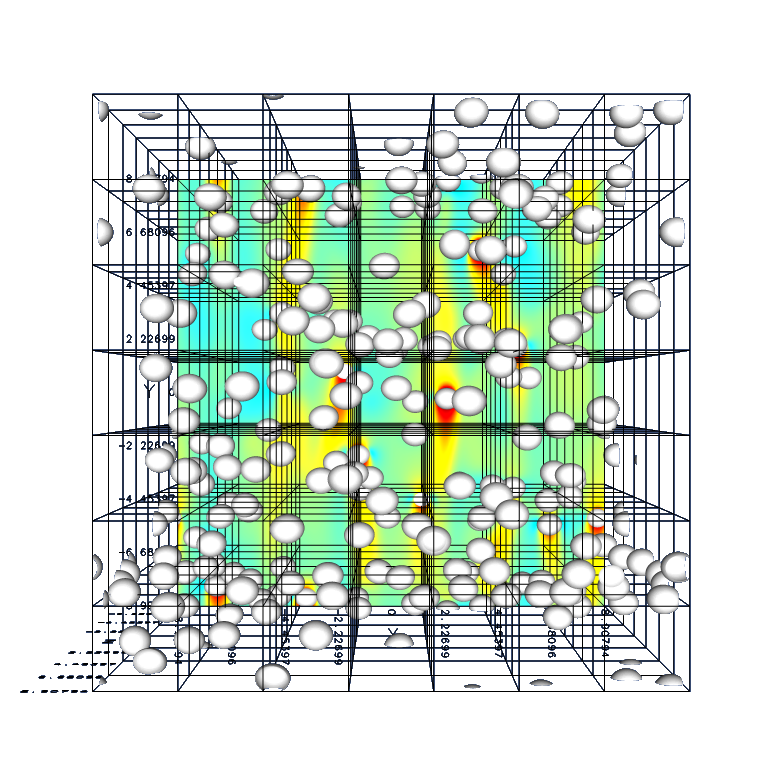
\includegraphics[width =  1.1\textwidth]{image/PHI_01_Ga_75.png}
\end{columns}
\end{frame}

\begin{frame}
  \frametitle{Direct Numerical Simulation of buoyant emulsions}
  \begin{columns}
    \column{0.6\textwidth}
  \underline{Dimensionless parameters :} 
  \begin{itemize}
    \item \textit{Galileo} number : $Ga =\frac{\sqrt{\rho \Delta\rho gD^3}}{\mu} \in [5, 100]$
    \item \textit{Bond} number : $Bo = \frac{\Delta \rho g D^2}{\sigma} = 1$ 
    \item volume fraction of dispersed phase : $\phi = [0.01;0.15]$. 
    \item Density and viscosity ratio, $\rho_r=1.11$ and $\mu_r= 0.1$. 
  \end{itemize}
  
  \begin{figure}
    \caption{Snapshot of a simulation at $T_g = 300$ for $\phi = 0.01$, $Ga = 75$ $\mu_r = 0.1$ and $N_b = 125$. In white : the interfaces, The background color map correspond to the pressure field. The grid represents the different core ($\le 729$ !).
    }
  \end{figure}
  \column{0.5\textwidth}
  \centering
  \href{file:///work/fintzin/BUBLLES_PROJECT/movies/cut.gif}{\beamergotobutton{Play}}
  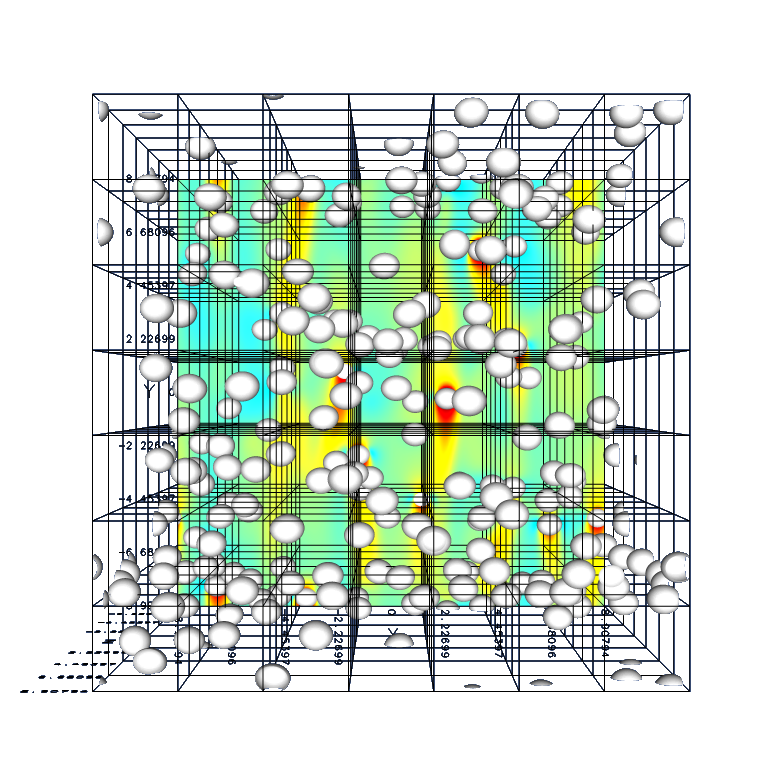
\includegraphics[width =  1.1\textwidth]{image/PHI_01_Ga_75.png}
  \end{columns}
\end{frame}

\begin{frame}
  \frametitle{Nearest pair probability density function}

  \begin{columns}
    \column{0.7\textwidth}
    \centering
    \begin{tabular}{cccc}
      &
      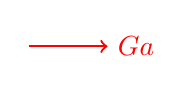
\begin{tikzpicture}[color=red]
        \draw[thick,->] (0,0) -- (1,0)node[right]{$Ga$};
      \end{tikzpicture}& & \\ 
        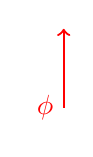
\begin{tikzpicture}[color=red]
          \draw[thick,<-] (0,0) -- (0,-1)node[left]{$\phi$};
        \end{tikzpicture} 
        &
        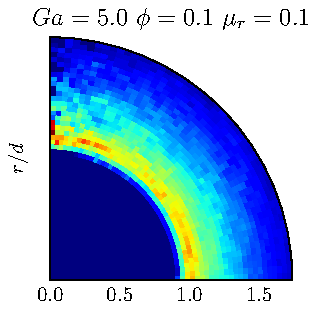
\includegraphics[height=0.3\textwidth]{image/HOMOGENEOUS/fDrop/Pnst_mu_r_0_1_Ga_5_PHI_0_1.pdf}  &
        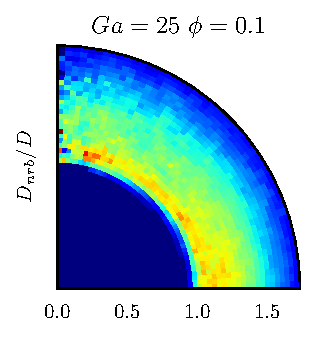
\includegraphics[height=0.3\textwidth]{image/HOMOGENEOUS/fDrop/Pnst_mu_r_0_1_Ga_25_PHI_0_1.pdf} &
        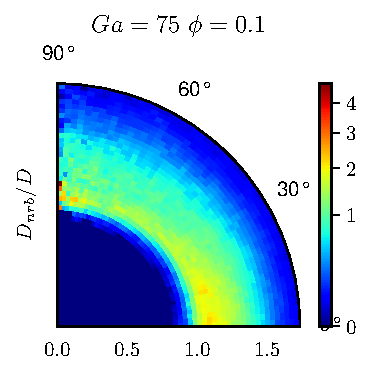
\includegraphics[height=0.3\textwidth]{image/HOMOGENEOUS/fDrop/Pnst_mu_r_0_1_Ga_75_PHI_0_1.pdf} 
        \\
         &
          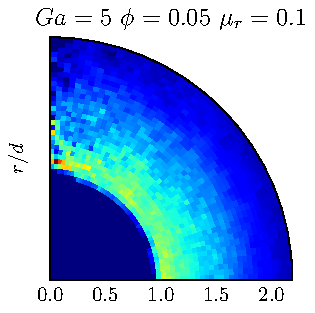
\includegraphics[height=0.3\textwidth]{image/HOMOGENEOUS/fDrop/Pnst_mu_r_0_1_Ga_5_PHI_0_05.pdf} &
        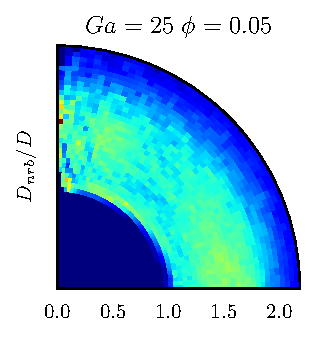
\includegraphics[height=0.3\textwidth]{image/HOMOGENEOUS/fDrop/Pnst_mu_r_0_1_Ga_25_PHI_0_05.pdf}&
        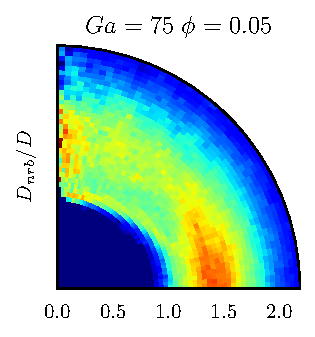
\includegraphics[height=0.3\textwidth]{image/HOMOGENEOUS/fDrop/Pnst_mu_r_0_1_Ga_75_PHI_0_05.pdf}\\
      \end{tabular}

      \column{0.3\textwidth}
      \begin{figure}
        \caption{Plots of $P_{nst} (\textbf{r})$ for different $Ga$ and $\phi$.}
      \end{figure}
    
    \begin{itemize}
      \item Drafting -Kissing tumbling mechanism for low $\phi$ and high $Ga$. 
    \end{itemize}
  \end{columns}
\end{frame}

\begin{frame}
  \frametitle{Reconstruction of the nearest relative velocity fields}

  \begin{figure}
    
    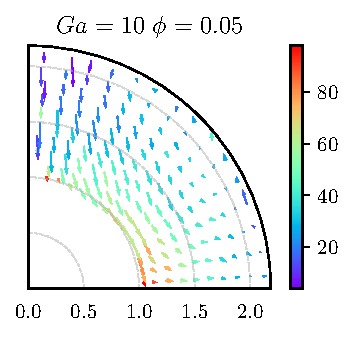
\includegraphics[height=0.25\textwidth]{image/HOMOGENEOUS/fDrop/U_mu_r_0_1_Ga_10_PHI_0_05.pdf}
    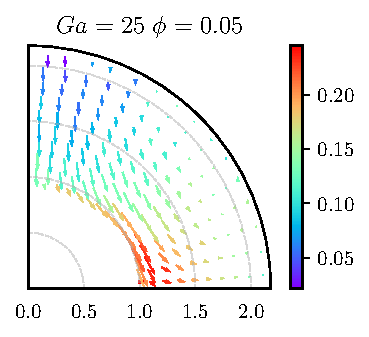
\includegraphics[height=0.25\textwidth]{image/HOMOGENEOUS/fDrop/U_mu_r_0_1_Ga_25_PHI_0_05.pdf}
    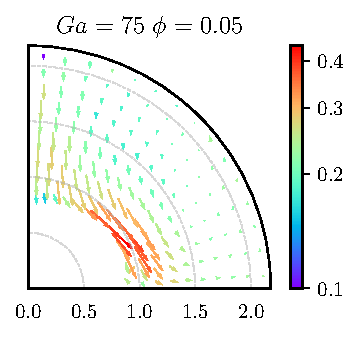
\includegraphics[height=0.25\textwidth]{image/HOMOGENEOUS/fDrop/U_mu_r_0_1_Ga_75_PHI_0_05.pdf}
    
    \caption{Nearest averaged velocity fields, $\nstavg{\textbf{w}} (\textbf{r})$ for different $Ga$ and $\phi$. 
    Colormap : magnitude of the relative velocity $|\nstavg{\textbf{w}}|$. }
  \end{figure}

\begin{itemize}
  \item In average particles approach from the top and leave through the sides. 
  % \item How to quantify this phenomenon ? 
  \item Representation of the Drafting -Kissing tumbling mechanism since the velocity fields converge toward high density zone. 
\end{itemize}
\end{frame}

\begin{frame}{The averaged nearest relative velocity equation}
  \begin{equation}
      \pddt P_{nst}
      + \frac{\partial}{\partial\textbf{x}} \cdot
      \left(
        \nstavg{\textbf{u}}
        P_{nst}
      \right)
      + \frac{\partial}{\partial\textbf{u}} \cdot
      \left(
        \nstavg{\textbf{a}}
        P_{nst}
      \right)
    + 
    \frac{\partial}{\partial \textbf{r}} \cdot
    \left(
        \nstavg{\textbf{w}}
        P_{nst}
    \right)
    = \Psi
    \label{eq:dt_P_nst1}
\end{equation}
Multiplying Eq. (\ref{eq:dt_P_nst1}) by \textbf{rr}, yields :
%  the \textbf{Mean square particles distance conservation equation  :}
\begin{equation}
  \pddt (\pavg{\textbf{R}})
  + \frac{\partial}{\partial\textbf{x}} \cdot
  (\pavg{\textbf{uR}})
  = 2\pavg{\textbf{P}}
  + \int \textbf{rr} \Psi d\textbf{r}
\end{equation}

\begin{itemize}
  \item $\textbf{R} = \int \textbf{rr} P_{nst} d\textbf{r}$ Mean square distance to the nearest particle. 
  \item $\textbf{P} = \int \textbf{r} \nstavg{\textbf{w}} P_{nst} d\textbf{r}$ correlation between $\nstavg{\textbf{w}}$ and $\textbf{r}$. 
  % \item $\int \textbf{rr} \dot{P_{nst}} d\textbf{r}$  source term tensor, still accounting for coalesces and breakup. 
\end{itemize}

$\rightarrow $ \textbf{R} is the mathematical representation of the mesoscale structures (cluster \ldots)
$\rightarrow $ The evolution of \textbf{R}, is proportional to \textbf{P}.
\end{frame}

\begin{frame}
  \frametitle{Computation of the correlation tensor $\avg{\nstavg{\textbf{rw}}}$ }
  \begin{figure}
    \begin{centering}
      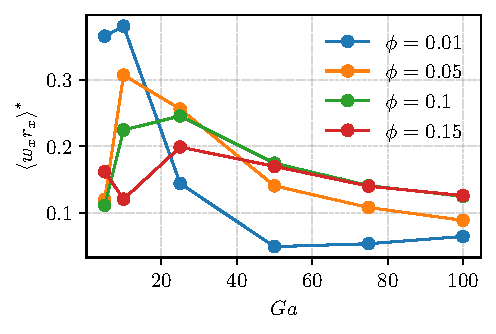
\includegraphics[height=0.25\textwidth]{image/HOMOGENEOUS/fPA/URxx.pdf}
      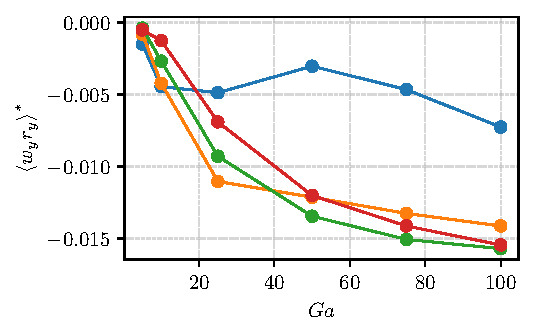
\includegraphics[height=0.25\textwidth]{image/HOMOGENEOUS/fPA/URyy.pdf}
      % 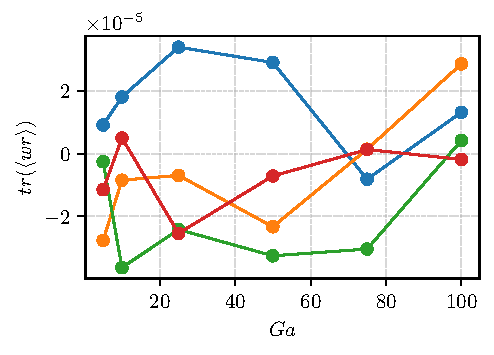
\includegraphics[height=0.2\textwidth]{image/HOMOGENEOUS/fPA/UR.pdf}
      \caption{Dimensionless correlation tensor $\avg{\textbf{r}\nstavg{\textbf{w}}} =  \int \textbf{r}\nstavg{\textbf{w}} P_{nst}(\textbf{x},\textbf{r})d\textbf{r}$}
    \end{centering}
  \end{figure}

  \begin{itemize}
    \item $r_x\nstrelavg{u_x} > 0$ \textbf{outward} particle flux.  
    \item $r_y\nstrelavg{u_y} < 0$ \textbf{inward} particle flux. 
    \item $\text{tr}\left(\textbf{r}\nstavg{\textbf{w}}\right) = 0$ conservation of the number of the nearest particle flux. 
  \end{itemize} 
\end{frame}


\begin{frame}
  \frametitle{Representation of the interaction force}

  \begin{figure}
    % 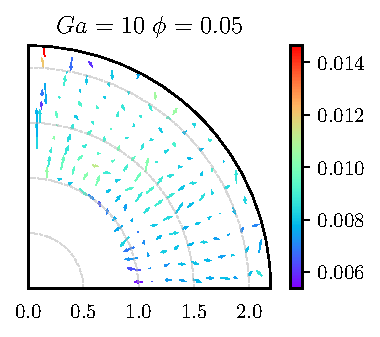
\includegraphics[height=0.25\textwidth]{image/HOMOGENEOUS/fDrop/F_mu_r_0_1_Ga_10_PHI_0_05.pdf}
    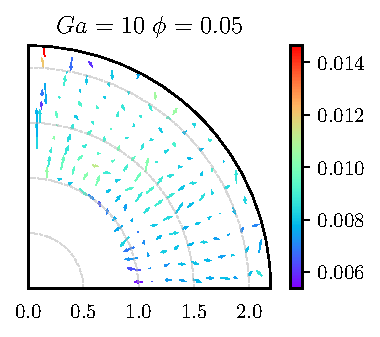
\includegraphics[height=0.25\textwidth]{image/HOMOGENEOUS/fDrop/F_mu_r_0_1_Ga_10_PHI_0_05.pdf}
    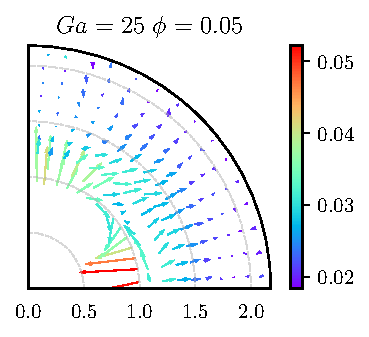
\includegraphics[height=0.25\textwidth]{image/HOMOGENEOUS/fDrop/F_mu_r_0_1_Ga_25_PHI_0_05.pdf}
    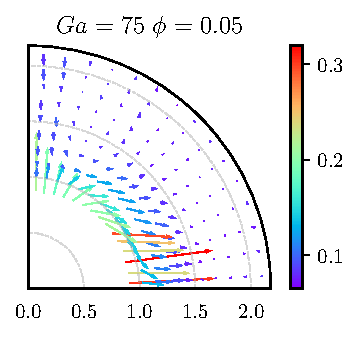
\includegraphics[height=0.25\textwidth]{image/HOMOGENEOUS/fDrop/F_mu_r_0_1_Ga_75_PHI_0_05.pdf}
    
    \caption{Nearest averaged relative acceleration fields times the mass of a particle. 
    Color map : Magnitude of the dimensionless force  $\nstrelavg{\textbf{F}} / (\Delta \rho V g)$.}
  \end{figure}

  
\begin{itemize}
  \item $\nstrelavg{\textbf{F}}$ is an isotropic repulsion force at high $Ga$. 
  \item At lower $Ga$ we observe attraction forces $\nstrelavg{\textbf{F}}$ on the sides.
\end{itemize}
$\rightarrow$ How to quantify these fields ? 
\end{frame}




\begin{frame}{The averaged nearest relative momentum equation}
  
  Multiplying the transport equation of $P_{nst}$ by \textbf{rw}, yields the transport equation of $\textbf{P}$, 
  % and integrating  over  all  \textbf{r} and \textbf{w} yields the \textbf{Mean relative momentum correlation equation :}
  
  
  \begin{equation*}
    \pddt (\pavg{\textbf{P}})
    + \frac{\partial}{\partial\textbf{x}} \cdot
    (\pavg{\textbf{uP}})
    = 2\pavg{\textbf{w}\nstavg{\textbf{w}}}
    + \mathbf{\Sigma}_{PFP}
    + \mathbf{\Sigma}_{B}
    + \int \textbf{ru} \Psi d\textbf{r}d\textbf{w}
  \end{equation*}
  
  \begin{itemize}
      \item $\textbf{P} = \int \textbf{r} \nstavg{\textbf{w}} P_{nst} d\textbf{r}$ correlation between the relative velocity $\nstavg{\textbf{w}}$ and $\textbf{r}$. 
    \item $\mathbf{\Sigma}_{PFP} = \int \textbf{r} \nstavg{\textbf{F}} P_{nst} d\textbf{r}d\textbf{w}$ correlation between \textbf{r} and the hydrodynamic  drag force on the particle $\nstavg{\textbf{F}}$. (\citet{zhang2021ensemble} : \textbf{particle stress})
    \item $\mathbf{\Sigma}_{B} = \int \textbf{r} \nstrelavg{\textbf{b}} P_{nst} d\textbf{r}d\textbf{w} = 0$, correlation between \textbf{r} and the \textbf{relative body} forces applied on the pair of nearest particles.
  \end{itemize}
  
  $\rightarrow$  Direct link between the relative velocities' tensor \textbf{P} and the relative hydrodynamic and body forces correlation, respectively $\Sigma_{PFP}$ and $\Sigma_B$.
  \end{frame}
  

\begin{frame}
  \frametitle{Computation of the particle stress}
  \underline{What is the particle stress (Zhang, JFM, 2021) ?}  
   : $\avg{\text{Drag Force}} = \avg{F} + \nablab \cdot \Sigma_{PFP}$
  \begin{figure}
    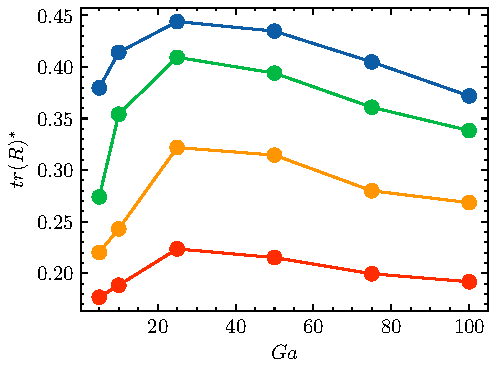
\includegraphics[height=0.25\textwidth]{image/HOMOGENEOUS/fPA/RR.pdf}
    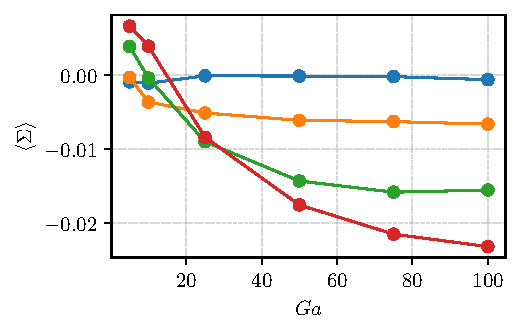
\includegraphics[height=0.25\textwidth]{image/HOMOGENEOUS/fPA/PFP.pdf}
    \caption{ 
      (left) Dimensionless  mean square distance to the nearest neighbor. 
      (right) Particle stress $\mathbf{\Sigma}_{PFP} = \int \textbf{r}\nstavg{\textbf{f}} P_{nst}d\textbf{r}$.
      }
  \end{figure}
  
\begin{itemize}
  \item $\text{tr}(\mathbf{\Sigma}_{PFP}) < 0$ global repulsion for high $\phi$ and $Ga$. 
  \item $\text{tr}(\mathbf{\Sigma}_{PFP}) > 0$ global attraction for small $Ga$ and $\phi$.
  % \item $\text{tr}(\mathbf{\Sigma}_{PFP}) = 0$ no pressure, when $\phi \rightarrow 0$ and $Ga \rightarrow 0$. 
  \item  $\mathbf{\Sigma}_{PFP}$ is directly correlated with the mean nearest particle distance $\textbf{R}$. 
\end{itemize}

\end{frame}


\section{First glimpse of coalescence modeling}
\section*{}

\begin{frame}
  \frametitle{Film drainage models to predict coalescence.}
  \begin{columns}
    \column{0.3\textwidth}
    \centering
    \begin{figure} 
      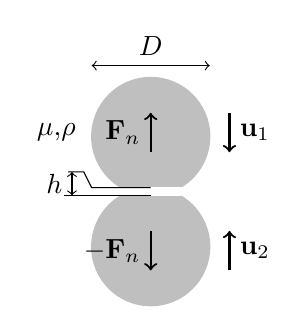
\begin{tikzpicture}
        \draw[lightgray,fill = lightgray] (0,0.7) circle (0.75);
        \draw[lightgray,fill = lightgray] (0,-0.7) circle (0.75);
        \draw[white,fill=white] (-0.75,-0.05) rectangle (0.75,0.05);
        \draw(0,0.05)--++(-0.75,0)--++(-0.1,0.2)--++(-0.2,0);
        \draw(0,-0.05)--++(-1.1,0);
        \draw[<->](-1,-0.05) --++ (0,0.3)node[midway,left]{$h$};
        \draw[<->](-0.75,1.6)--++(1.5,0)node[midway,above]{$D$};
        \node (para) at (-1.2,0.75){$\mu$,$\rho$};
        \draw[->,thick](0,0.5)--++(0,0.5)node[midway,left]{$\textbf{F}_n$};
        \draw[->,thick](0,-0.5)--++(0,-0.5)node[midway,left]{$-\textbf{F}_n$};
        \draw[<-,thick](1,0.5)--++(0,0.5)node[midway,right]{$\textbf{u}_1$};
        \draw[<-,thick](1,-0.5)--++(0,-0.5)node[midway,right]{$\textbf{u}_2$};
      \end{tikzpicture}
      \caption{Scheme of two colliding droplets.}
    \end{figure}
    \column{0.7\textwidth}
    \begin{columns}[t]
      \column{0.5\textwidth}
      \textbf{Current film thickness : }  
      \begin{equation*}
        \frac{h(t_c,F_n)}{D}  \sim \frac{\textcolor{red}{F_n} \mu^{1/2}}{\textcolor{red}{t_c} \sigma} 
      \end{equation*}
      \begin{itemize}
        \item \underline{$F_n$ : Interaction force}
        \item $D$ : Droplets diameters
        \item $\sigma$ : Surface tension coefficient
        \item \underline{$t_c$ : contact time}
      \end{itemize}
      \citet{chesters1991modelling}
      \column{0.5\textwidth}
      \textbf{Critical thickness \footnote{\citet{yoon2007coalescence}}} 
      \begin{equation*}
        \frac{h_c}{D} \sim  \frac{A_HCa^{1/6}}{\sigma^{1/3}} 
      \end{equation*}
      \begin{itemize}
        \item $Ca$ : Capillary number 
        \item $A_H = 2.4\cdot 10^{-21}$ : Hamaker constant
      \end{itemize}
    \end{columns}
  \end{columns}
  \vfill
  \begin{itemize}
    \item How to estimate $\textcolor{red}{F_n}$ and $\textcolor{red}{t_c}$ ? 
  \end{itemize}
\end{frame}


\begin{frame}
  \frametitle{Prediction of $F_n$ and $t_c$ with DNS results.}
  \begin{columns}
    \column{0.3\textwidth}
    \centering
    \begin{figure} 
      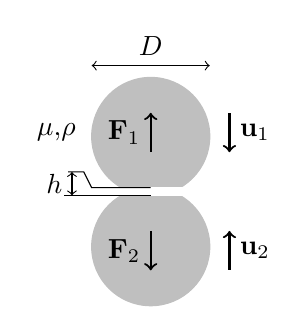
\begin{tikzpicture}
        \draw[lightgray,fill = lightgray] (0,0.7) circle (0.75);
        \draw[lightgray,fill = lightgray] (0,-0.7) circle (0.75);
        \draw[white,fill=white] (-0.75,-0.05) rectangle (0.75,0.05);
        \draw(0,0.05)--++(-0.75,0)--++(-0.1,0.2)--++(-0.2,0);
        \draw(0,-0.05)--++(-1.1,0);
        \draw[<->](-1,-0.05) --++ (0,0.3)node[midway,left]{$h$};
        \draw[<->](-0.75,1.6)--++(1.5,0)node[midway,above]{$D$};
        \node (para) at (-1.2,0.75){$\mu$,$\rho$};
        \draw[->,thick](0,0.5)--++(0,0.5)node[midway,left]{$\textbf{F}_1$};
        \draw[->,thick](0,-0.5)--++(0,-0.5)node[midway,left]{$\textbf{F}_2$};
        \draw[<-,thick](1,0.5)--++(0,0.5)node[midway,right]{$\textbf{u}_1$};
        \draw[<-,thick](1,-0.5)--++(0,-0.5)node[midway,right]{$\textbf{u}_2$};
      \end{tikzpicture}
      \caption{Scheme of two colliding droplets labeled $1$ and $2$.}
    \end{figure}
    \column{0.7\textwidth}
    \begin{columns}
      \column{0.5\textwidth}
      \centering
      \begin{figure}
        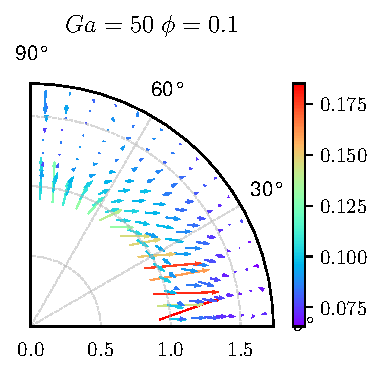
\includegraphics[width=0.9\textwidth]{image/HOMOGENEOUS/fDrop/F_mu_r_0_1_Ga_50_PHI_0_1.pdf}
        \caption{Nearest relative averaged force fields, $\nstrelavg{\textbf{F}}(\textbf{r})$.}
      \end{figure}
      \column{0.5\textwidth}
      \centering
      \begin{figure}
      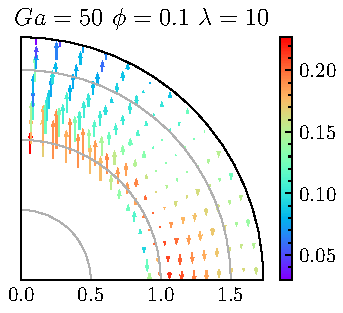
\includegraphics[width=0.9\textwidth]{image/HOMOGENEOUS/fDrop/U_mu_r_0_1_Ga_50_PHI_0_1.pdf}
      \caption{Relative averaged velocity fields, $\nstavg{\textbf{w}}(\textbf{r})$.}
    \end{figure}
    \end{columns}
  \end{columns}
  \begin{itemize}
    \item We notice that $F_c$ and $t_c$ are function of \textbf{r}, $\phi$, $Ga$, $\mu_r$ \ldots
    \item Therefore,
    $ h(t_c,F_n,\textbf{r})  \sim F_n(\textbf{r}) / t_c(\textbf{r}) D \sigma^{-1} \mu^{1/2}$
  \end{itemize}
\end{frame}

\begin{frame}
  \frametitle{Motion and coalesce of the nearest droplet}
\centering
\begin{tikzpicture}
  \node (img) at (0,0) {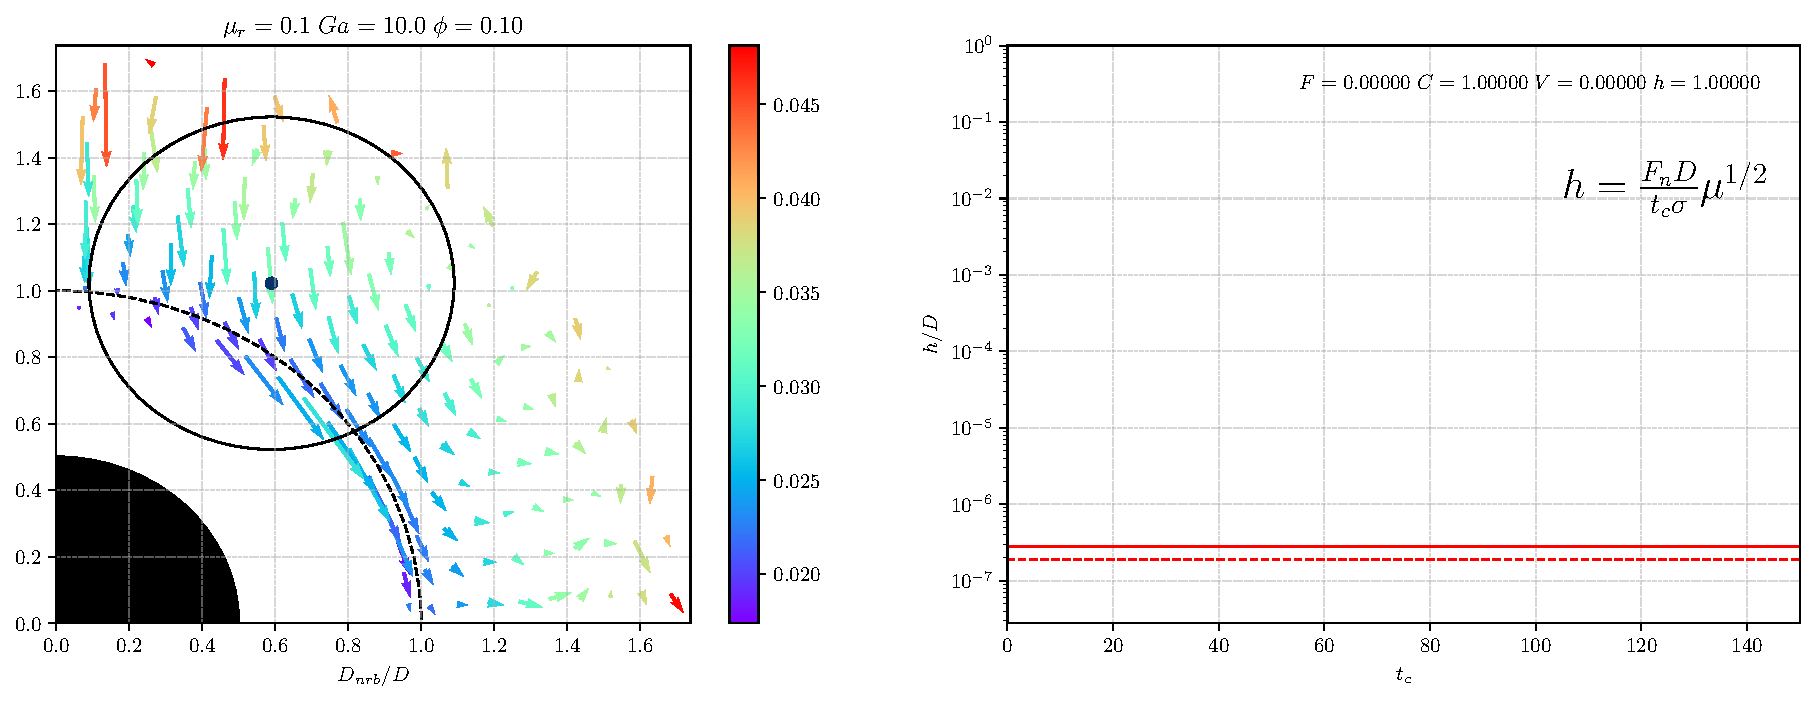
\includegraphics[width=\textwidth]{image/HOMOGENEOUS/anim/frame_1_0_1_Ga_10_PHI_0_1.pdf}};
  \node (hc) at (1.4,-1.8) {\textcolor{red}{$h_c$}};
\end{tikzpicture}
  % \includegraphics[width=\textwidth]{../movies/P_PHI_1_Ga_75.gif}
  
  $Ga = 10$ :
  \href{file:///work/fintzin/BUBLLES_PROJECT/movies/First_anim.mp4}{\beamergotobutton{Play}}\\
  $Ga = 25$ :
  \href{file:///work/fintzin/BUBLLES_PROJECT/results/HOMOGENEOUS/Dim_3/N_5/PHI_0.1/rho_r_1.11/Bo_1/mu_r_0.1/Ga_25/animation_N1.mp4}{\beamergotobutton{Play}}\\
  $Ga = 50$ :
  \href{file:///work/fintzin/BUBLLES_PROJECT/results/HOMOGENEOUS/Dim_3/N_5/PHI_0.1/rho_r_1.11/Bo_1/mu_r_0.1/Ga_50/animation_N1.mp4}{\beamergotobutton{Play}}
\end{frame}

\begin{frame}
  \frametitle{Motion and coalesce of the nearest droplets }
\centering
  \begin{tikzpicture}
    \node (img) at (0,0) {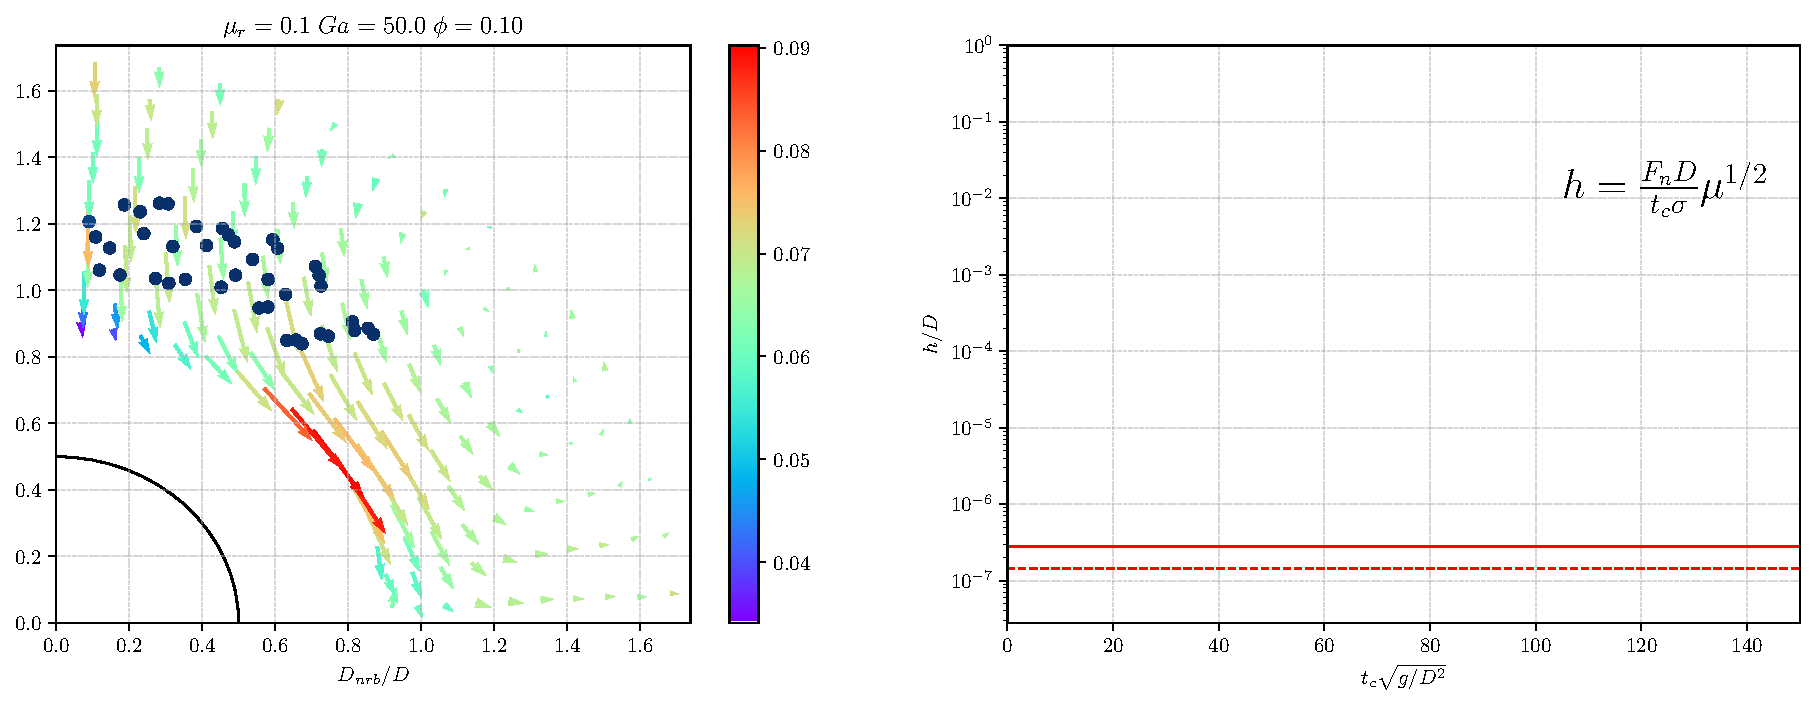
\includegraphics[width=\textwidth]{image/HOMOGENEOUS/anim/frame_1_N40_0_1_Ga_50_PHI_0_1.pdf}};
    \node (hc) at (1.4,-1.8) {\textcolor{red}{$h_c$}};
  \end{tikzpicture}
  % \href{file:///work/fintzin/BUBLLES_PROJECT/results/HOMOGENEOUS/Dim_3/N_5/PHI_0.1/rho_r_1.11/Bo_1/mu_r_0.1/Ga_25/animation_N1.mp4}{\beamergotobutton{Play}}
  
  \begin{columns}
    \column{0.5\textwidth}
    \centering
    \begin{tabular}{|c|c|c|}\hline
       &
      $Ga = 10$ &
      \href{file:///work/fintzin/BUBLLES_PROJECT/results/HOMOGENEOUS/Dim_3/N_5/PHI_0.1/rho_r_1.11/Bo_1/mu_r_0.1/Ga_10/animation.mp4}{\beamergotobutton{Play}}\\
      $\phi = 0.1$&
      $Ga = 25$ &
      \href{file:///work/fintzin/BUBLLES_PROJECT/results/HOMOGENEOUS/Dim_3/N_5/PHI_0.1/rho_r_1.11/Bo_1/mu_r_0.1/Ga_25/animation.mp4}{\beamergotobutton{Play}}\\
      &
      $Ga = 50$ &
      \href{file:///work/fintzin/BUBLLES_PROJECT/results/HOMOGENEOUS/Dim_3/N_5/PHI_0.1/rho_r_1.11/Bo_1/mu_r_0.1/Ga_50/animation.mp4}{\beamergotobutton{Play}}\\\hline
    \end{tabular}
    \column{0.5\textwidth}
    \centering
    \begin{tabular}{|c|c|c|}\hline
      &
     $Ga = 10$ &
     \href{file:///work/fintzin/BUBLLES_PROJECT/results/HOMOGENEOUS/Dim_3/N_5/PHI_0.01/rho_r_1.11/Bo_1/mu_r_0.1/Ga_10/animation.mp4}{\beamergotobutton{Play}}\\
     $\phi = 0.01$&
     $Ga = 25$ &
     \href{file:///work/fintzin/BUBLLES_PROJECT/results/HOMOGENEOUS/Dim_3/N_5/PHI_0.01/rho_r_1.11/Bo_1/mu_r_0.1/Ga_25/animation.mp4}{\beamergotobutton{Play}}\\
     &
     $Ga = 50$ &
     \href{file:///work/fintzin/BUBLLES_PROJECT/results/HOMOGENEOUS/Dim_3/N_5/PHI_0.01/rho_r_1.11/Bo_1/mu_r_0.1/Ga_50/animation.mp4}{\beamergotobutton{Play}}\\\hline
   \end{tabular}
  \end{columns}
\end{frame}

\section{Conclusion and discussion}
\section*{}
\begin{frame}
  \frametitle{General remarks and conclusion}

  \begin{itemize}
    \item We used the nearest particle statistics to derive relative pair interactions equation. 
    \item We found out that relative velocity and forces are directly correlated to the relative position \textbf{r} with $Ga$ and $\phi$. 
    \item We predicted coalesce event in the different regime. 
  \end{itemize}
  \begin{columns}
    \column{0.6\textwidth}
    \underline{Future projects : }  
    
    \begin{itemize}
      \item Deriving semi empirical formulation for the coalescence kernel which takes in account the cinematic \textbf{P}, the dynamics $\mathbf{\Sigma}_{PFP}$, and the mean total time of interaction. 
    \end{itemize}
    \column{0.4\textwidth}
    \begin{figure}
      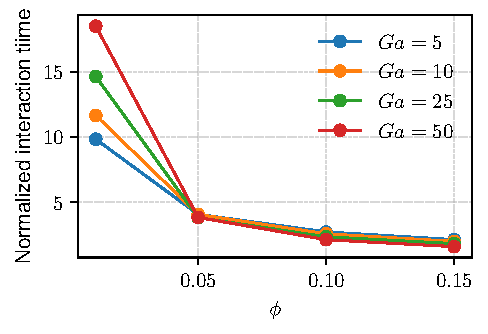
\includegraphics[width=\textwidth]{image/HOMOGENEOUS/fPA/age.pdf}
      % \caption{Normalized time of interaction}
    \end{figure}
  \end{columns}
    
% \vspace{1cm}
See my work : \url{http://basilisk.fr/sandbox/fintzin/Rising-Suspenion/}

\end{frame}

\begin{frame}
  \frametitle{Closure terms for the averaged Navier Stokes equation.}
\begin{columns}
  \begin{column}{0.5\textwidth}
    \begin{figure}
      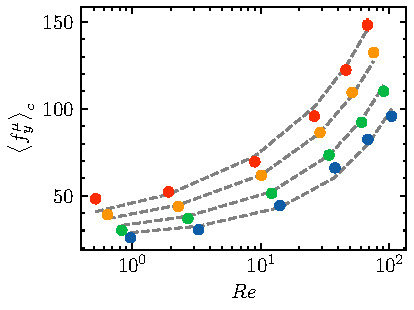
\includegraphics[width=0.7\textwidth]{image/HOMOGENEOUS/fCA/FH_mu_Re.pdf}
      \caption{Dimensionless drag force in terms $Re$ for $\phi = 0.01, 0.05, 0.1$ and $0.15$.}
    \end{figure}
    \begin{equation*}
      \frac{\avg{f}}{\mu UD} 
      = 1.18 e^{5.32\phi^{1/3}}  Re^{0.33}  + Re^{0.87} +24.12
    \end{equation*}
  \end{column}
  \begin{column}{0.5\textwidth}
    \begin{figure}[h!]
      \centering
      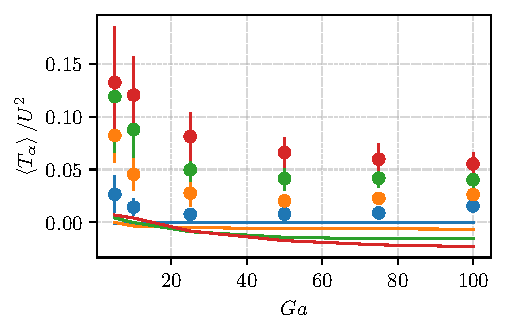
\includegraphics[width=0.7\textwidth]{image/HOMOGENEOUS/fPA/Talpha.pdf}
      \caption{Dimensionless granular temperature in terms of $Ga$ and $\phi$}
  \end{figure}
  	\begin{equation}
    \frac{\avg{\textbf{u}'\cdot \textbf{u}'}}{U^2}  
    \approx \frac{\phi}{Ga^2} 2.86\cdot10^{4} 
    \label{eq:Talpha_scaling}
	\end{equation}
    % \begin{itemize}
    %   \item $U$ is the relative velocity between the continuous and dispersed phase.
    %   \item $Re$ is the \textit{Reynolds} number defined as, $Re = \rho D U / \mu$. 
    % \end{itemize}
  \end{column}
\end{columns}

\end{frame}

\begin{frame}[t]
  \frametitle{References}
  \bibliography{Bib/bib_bulles.bib}
\end{frame}

 
\backmatter
\begin{frame}
  \frametitle{Computation of the damping ratio ? }
  \begin{figure}
    \centering
    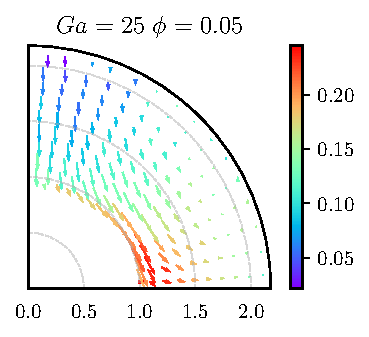
\includegraphics[width=0.27\textwidth]{image/HOMOGENEOUS/fDrop/U_mu_r_0_1_Ga_25_PHI_0_05.pdf}
    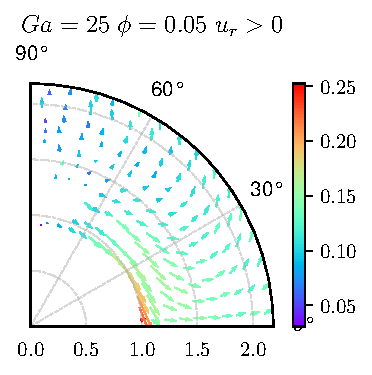
\includegraphics[width=0.27\textwidth]{image/HOMOGENEOUS/fDrop/Upos_mu_r_0_1_Ga_25_PHI_0_05.pdf}
    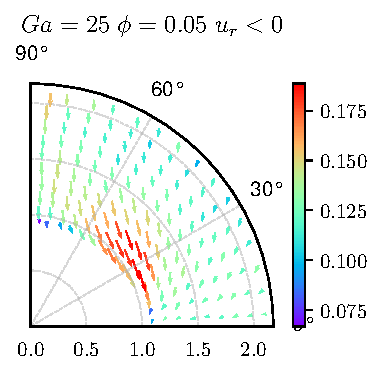
\includegraphics[width=0.27\textwidth]{image/HOMOGENEOUS/fDrop/Uneg_mu_r_0_1_Ga_25_PHI_0_05.pdf}
    \caption{Nearest averaged force fields, $\nstavg{\textbf{w}}(\textbf{r})$ for different $Ga$ and $\phi$. 
    Color map : Magnitude of the dimensionless force  $\nstavg{\textbf{w}} / (\Delta \rho V g)$.
    (middle) conditional average  $\nstrelavg{\textbf{u}| u_r > 0}(\textbf{r})$. 
    (right) conditional average  $\nstrelavg{\textbf{u}| u_r < 0}(\textbf{r})$ }
  \end{figure}
  \begin{equation}
    \text{Damping Ratio}
    \approx \frac{\avg{\frac{1}{2} \textbf{u} \cdot \textbf{u}| u_r > 0}}
    {\avg{\frac{1}{2}\textbf{u}\cdot \textbf{u}| u_r < 0}}
    = 0.12
  \end{equation}
\end{frame}

\begin{frame}
  \frametitle{Conditional average of the force on the velocity}
  \begin{figure}
    \centering
    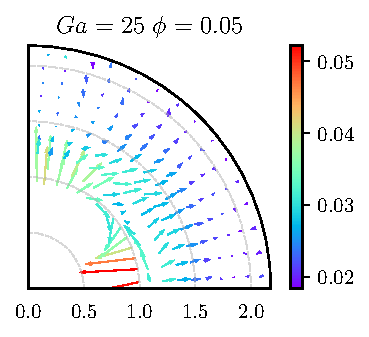
\includegraphics[width=0.33\textwidth]{image/HOMOGENEOUS/fDrop/F_mu_r_0_1_Ga_25_PHI_0_05.pdf}
    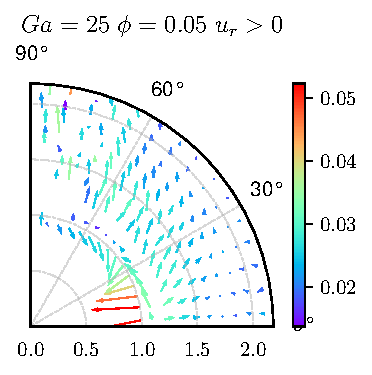
\includegraphics[width=0.33\textwidth]{image/HOMOGENEOUS/fDrop/Fpos_mu_r_0_1_Ga_25_PHI_0_05.pdf}
    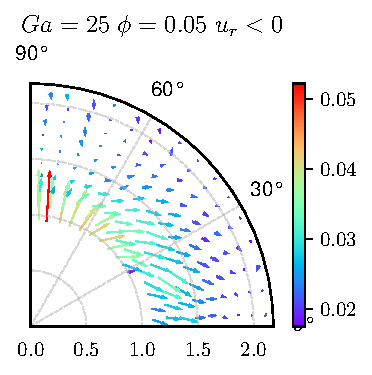
\includegraphics[width=0.33\textwidth]{image/HOMOGENEOUS/fDrop/Fneg_mu_r_0_1_Ga_25_PHI_0_05.pdf}
    \caption{Nearest averaged force fields, $\nstrelavg{\textbf{F}}(\textbf{r})$ for different $Ga$ and $\phi$. 
    Color map : Magnitude of the dimensionless force  $\nstrelavg{\textbf{F}} / (\Delta \rho V g)$.
    (middle) conditional average  $\nstrelavg{\textbf{F}| u_r > 0}(\textbf{r})$. 
    (right) conditional average  $\nstrelavg{\textbf{F}| u_r < 0}(\textbf{r})$ }
  \end{figure}
\end{frame}

\begin{frame}
  \frametitle{Conditional average of the force on the velocity}
  \begin{figure}
    \centering
    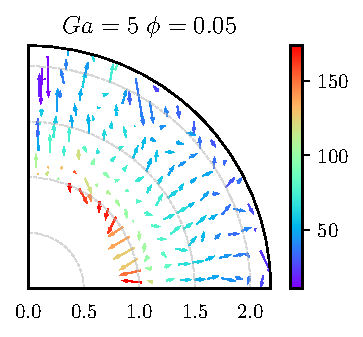
\includegraphics[width=0.33\textwidth]{image/HOMOGENEOUS/fDrop/F_mu_r_0_1_Ga_5_PHI_0_05.pdf}
    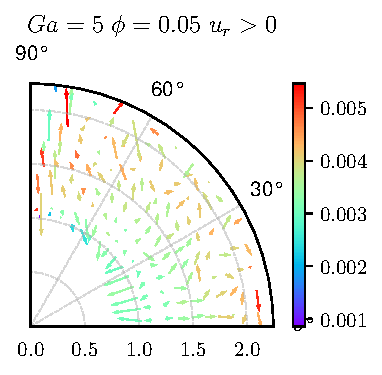
\includegraphics[width=0.33\textwidth]{image/HOMOGENEOUS/fDrop/Fpos_mu_r_0_1_Ga_5_PHI_0_05.pdf}
    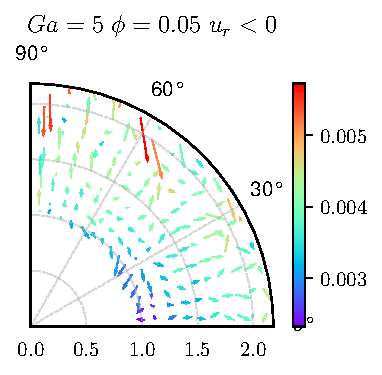
\includegraphics[width=0.33\textwidth]{image/HOMOGENEOUS/fDrop/Fneg_mu_r_0_1_Ga_5_PHI_0_05.pdf}
    \caption{Nearest averaged force fields, $\nstrelavg{\textbf{F}}(\textbf{r})$ for different $Ga$ and $\phi$. 
    Color map : Magnitude of the dimensionless force  $\nstrelavg{\textbf{F}} / (\Delta \rho V g)$.
    (middle) conditional average  $\nstrelavg{\textbf{F}| u_r > 0}(\textbf{r})$. 
    (right) conditional average  $\nstrelavg{\textbf{F}| u_r < 0}(\textbf{r})$ }
  \end{figure}
\end{frame}


  
\end{document}
